% Source of the figure square-decomposition.pdf: schematic of the square decomposition S_1, P_{1,1}, P_{1,2},
% S_2, ..., S_k of (G,u,v). Squares are boxes, links are ellipses, edges of F are dashed arrows from tail to head.
% Compile with pdfLaTeX; the PDF is included in the manuscript at its natural size.
\documentclass[tikz,border=1pt]{standalone}
\usepackage[T1]{fontenc}
\pdfinfoomitdate=1 \pdftrailerid{} \pdfsuppressptexinfo=-1
\usetikzlibrary{arrows.meta,shapes.geometric}
\definecolor{fblue}{RGB}{31,102,178}
\tikzset{
  vertex/.style={circle, fill=black, inner sep=0pt, minimum size=2.2mm},
  terminal/.style={circle, fill=black, inner sep=0pt, minimum size=3mm},
  square/.style={rounded corners=4pt, fill=gray!14, draw=gray!75!black, line width=0.9pt},
  link/.style={ellipse, fill=gray!32, draw=gray!75!black, line width=0.6pt, inner sep=0pt,
               minimum width=8mm, minimum height=5.5mm},
  fedge/.style={line width=0.9pt, fblue, dash pattern=on 3pt off 1.6pt, -{Stealth[length=2.4mm, width=2mm]}}}
\begin{document}
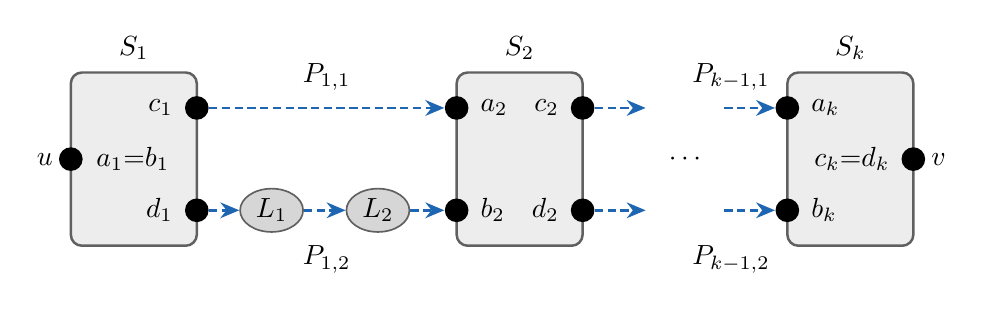
\begin{tikzpicture}[x=1cm, y=1cm]
  \def\h{1.1}   % half height of a square
  \def\t{0.65}  % vertical offset of the terminals
  % the squares S_1, S_2, S_k
  \draw[square] (0,-\h) rectangle (1.6,\h);
  \draw[square] (4.9,-\h) rectangle (6.5,\h);
  \draw[square] (9.1,-\h) rectangle (10.7,\h);
  \node[above=1pt] at (0.8,\h)  {$S_1$};
  \node[above=1pt] at (5.7,\h)  {$S_2$};
  \node[above=1pt] at (9.9,\h)  {$S_k$};
  % terminals
  \node[terminal] (u)  at (0,0) {};
  \node[terminal] (c1) at (1.6,\t) {};
  \node[terminal] (d1) at (1.6,-\t) {};
  \node[terminal] (a2) at (4.9,\t) {};
  \node[terminal] (b2) at (4.9,-\t) {};
  \node[terminal] (c2) at (6.5,\t) {};
  \node[terminal] (d2) at (6.5,-\t) {};
  \node[terminal] (ak) at (9.1,\t) {};
  \node[terminal] (bk) at (9.1,-\t) {};
  \node[terminal] (v)  at (10.7,0) {};
  \node[left=3pt]  at (u) {$u$};
  \node[right=3pt] at (v) {$v$};
  \node[anchor=west] at (0.2,0)     {$a_1{=}b_1$};
  \node[anchor=east] at (1.42,\t)   {$c_1$};
  \node[anchor=east] at (1.42,-\t)  {$d_1$};
  \node[anchor=west] at (5.08,\t)   {$a_2$};
  \node[anchor=west] at (5.08,-\t)  {$b_2$};
  \node[anchor=east] at (6.32,\t)   {$c_2$};
  \node[anchor=east] at (6.32,-\t)  {$d_2$};
  \node[anchor=west] at (9.28,\t)   {$a_k$};
  \node[anchor=west] at (9.28,-\t)  {$b_k$};
  \node[anchor=east] at (10.52,0)   {$c_k{=}d_k$};
  % P_{1,1}: a single edge of F
  \draw[fedge] (c1) -- (a2);
  \node[anchor=south] at (3.25,0.75) {$P_{1,1}$};
  % P_{1,2}: edge, link, edge, link, edge
  \node[link] (l1) at (2.55,-\t) {$L_1$};
  \node[link] (l2) at (3.9,-\t)  {$L_2$};
  \draw[fedge] (d1) -- (l1);
  \draw[fedge] (l1) -- (l2);
  \draw[fedge] (l2) -- (b2);
  \node[anchor=north] at (3.25,-0.98) {$P_{1,2}$};
  % the chain continues from S_2 to S_k
  \draw[fedge] (c2) -- ++(0.8,0);
  \draw[fedge] (d2) -- ++(0.8,0);
  \draw[fedge] (8.3,\t) -- (ak);
  \draw[fedge] (8.3,-\t) -- (bk);
  \node at (7.8,0) {$\cdots$};
  \node[anchor=south east] at (9.0,0.75) {$P_{k-1,1}$};
  \node[anchor=north east] at (9.0,-0.98) {$P_{k-1,2}$};
\end{tikzpicture}
\end{document}
